\appendix 
\section{Appendix}
% \balance
\label{sec:appendix}
\subsection{Components of Variation-aware Loss}
\label{app:loss}
1. \textbf{Amplitude Shifting Invariance}: Implemented using the softmax function to ensure that the gap between the prediction and the ground truth is equal at each step. The formula is as follows:
   \[
   \mathcal{L}_{\text{a.shift}}(Y, \hat{Y}) = \frac{1}{T'} \sum_{i=1}^{T'} \left| 1 - \text{Softmax}(d(y_i, \hat{y}_i)) \right|
   \]
   where \(d(y_i, \hat{y}_i)\) is the signed distance between the true value and the predicted value, and \(T'\) is the length of the sequence.

2. \textbf{Phase Shifting Invariance}: Achieved by utilizing the gap between the Fourier coefficients to retain the dominant frequency components of the original time series while reducing noise in non-dominant frequencies. The formula is as follows:
   \[
   \mathcal{L}_{\text{phase}}(Y, \hat{Y}) = \begin{cases} 
   \left\| F(Y) - F(\hat{Y}) \right\|_p & \text{for dominant freq.} \\
   \left\| F(\hat{Y}) \right\|_p & \text{otherwise}
   \end{cases}
   \]
   where \(F(Y)\) and \(F(\hat{Y})\) are the Fourier transforms of the true and predicted values, respectively, and \(\left\| \cdot \right\|_p\) is the Lp norm.

3. \textbf{Point-wise Distance}: Implemented through the mean average error to measure the average magnitude of the errors in a set of predictions, without considering their direction. The formula is as follows:
   \[
   \mathcal{L}_{\text{distance}}(Y, \hat{Y}) = \frac{1}{T'} \sum_{i=1}^{T'} \left| y_i - \hat{y}_i \right|
   \]
   where \(y_i\) and \(\hat{y}_i\) are the true and predicted values at time step \(i\), respectively, and \(T'\) is the length of the sequence.



\subsection{Spatio-temporal Periodicity.}
In this work, we develop a thermodynamic model of the urban heat island effect primarily using a historical spatio-temporal field temperature dataset. To manage the complex variations in thermal issues, we integrate thermal equations to guide our model and simplify the modeling process through an equation-based decomposition framework. We introduce the design of each component from a thermal modeling perspective and demonstrate their effectiveness in the paper. 

\begin{figure*}[!t]
    \centering
    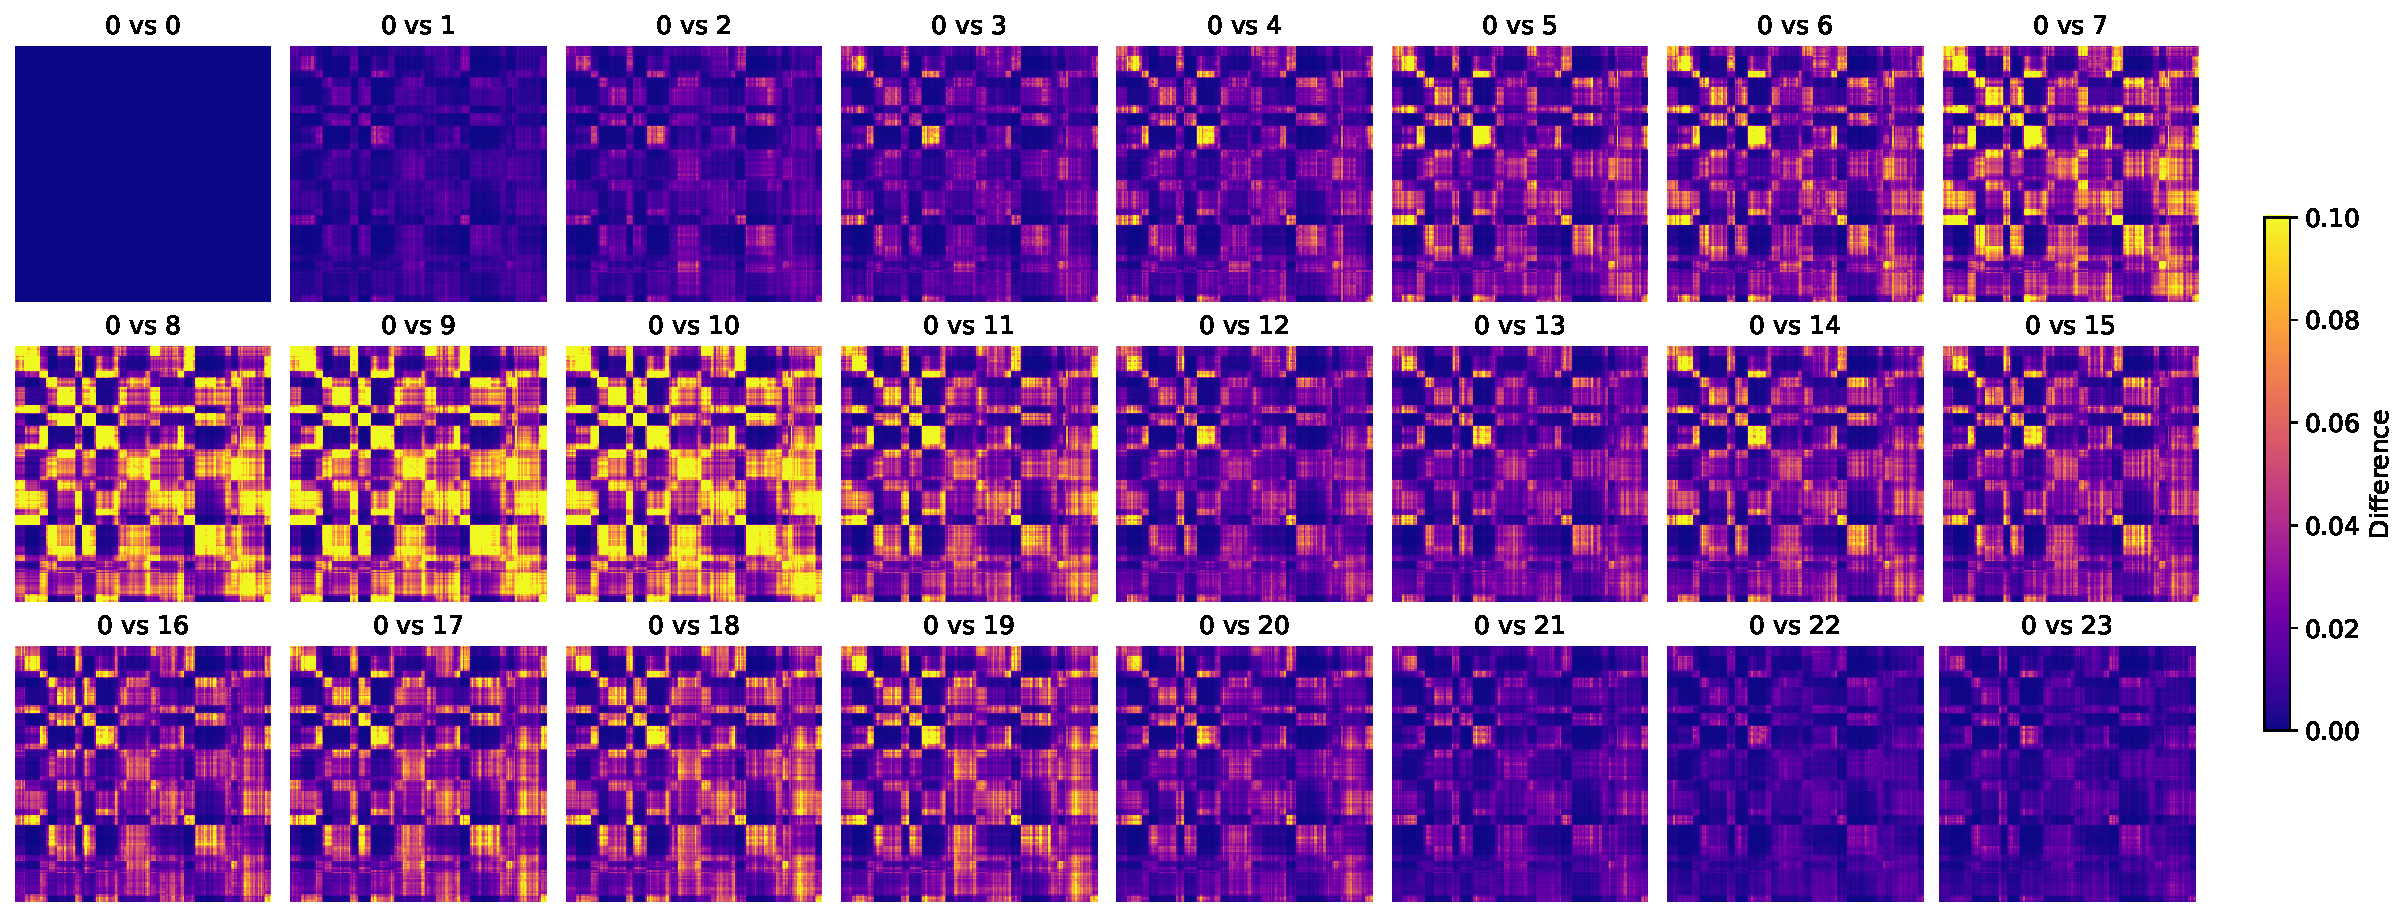
\includegraphics[width=0.95\linewidth]{resources/flow_cycle.pdf}
    \vspace{-1em}
    \caption{Spatio-relation Periodicity: daily variation of the learned adjacency matrix}
    \label{fig:flow_cycle}
\end{figure*}

However, from a data-driven spatio-temporal forecasting perspective, some parameter designs based on thermal principles may still require further experimental validation. Specifically, our model is designed to leverage the spatio-temporal periodicity of field temperature data. Below, we will present additional experimental evidence regarding the spatio-temporal periodicity of temperature data.


\begin{figure}[!h]
    \centering
    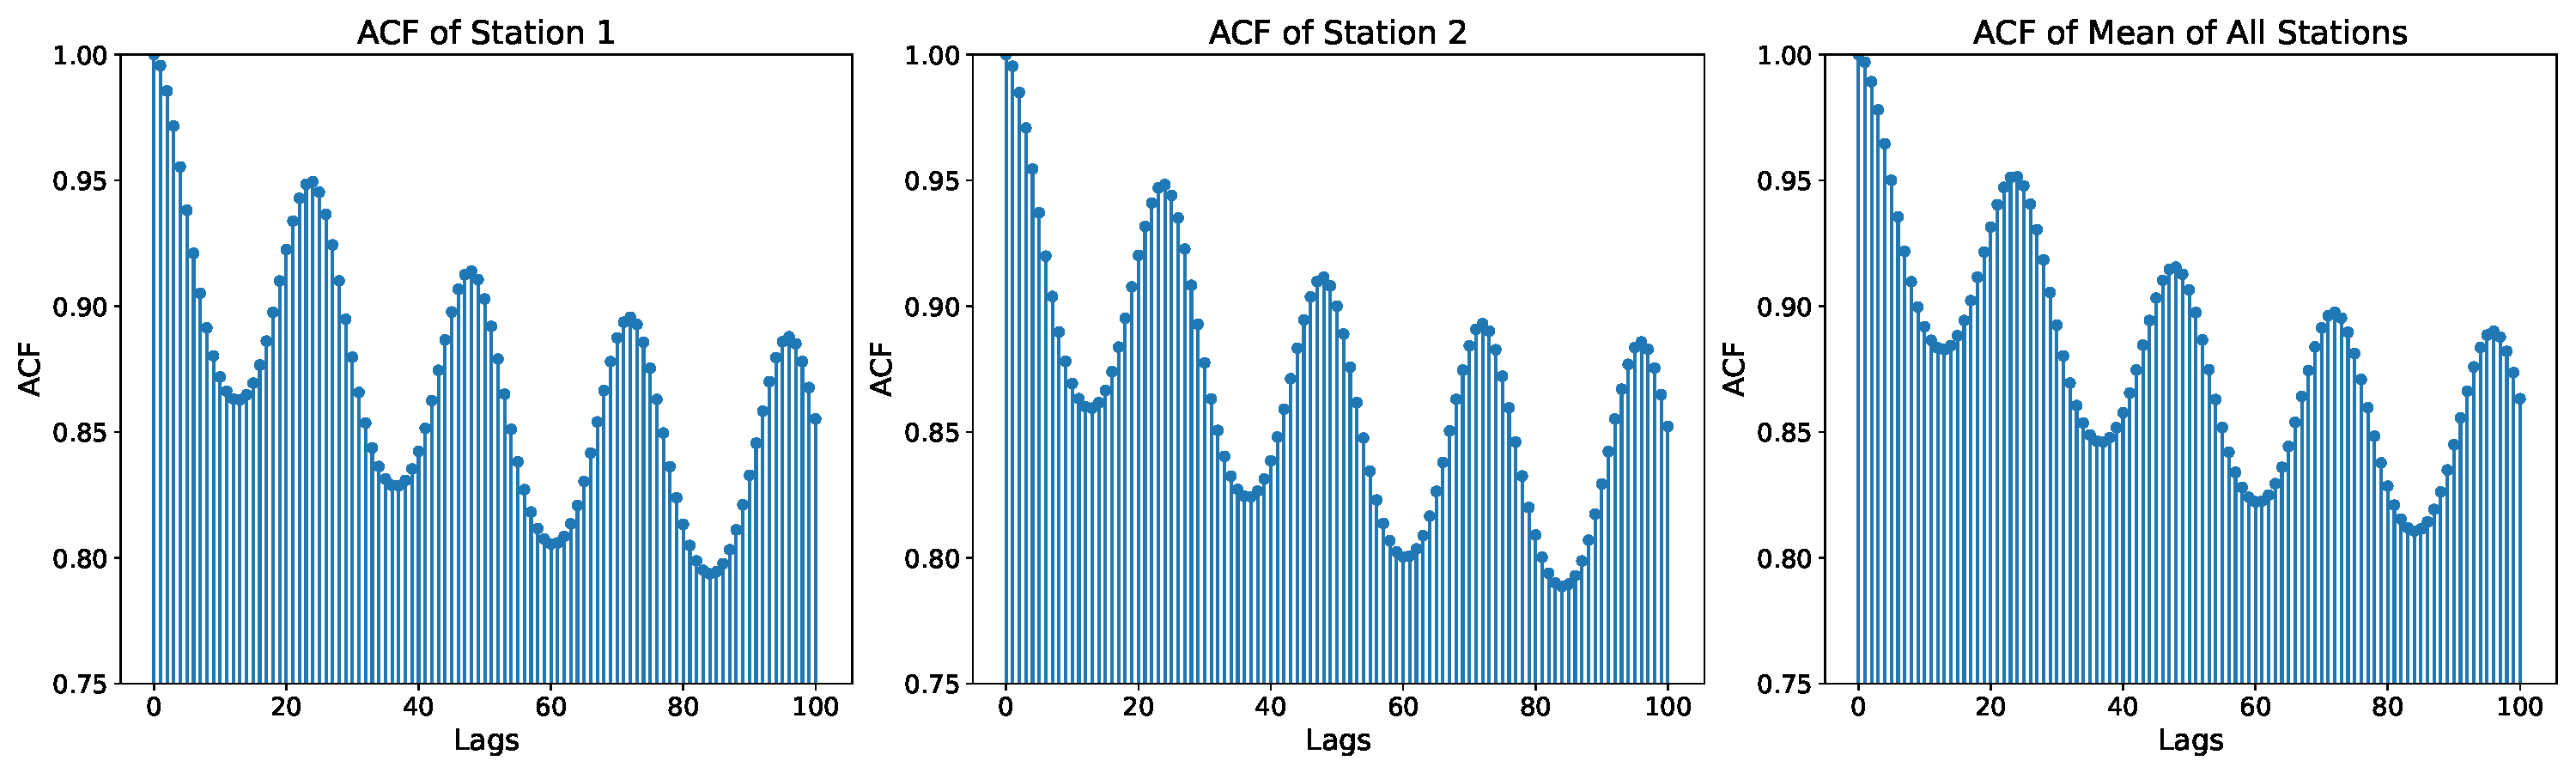
\includegraphics[width=0.95\linewidth]{resources/ACF.pdf}
    \caption{Intra-region Temporal Periodicity: visualization of ACF results on \textit{SeoulTemp} Dataset}
    \label{fig:acf}
\end{figure}

\textbf{Spatio-relation Periodicity.} In Section \ref{sec:spatial_cycle}, we efficiently model the temporal periodic dynamics of \textbf{thermal flow} by setting a period \underline{$W=24$ (daily)}. This approach simplifies the modeling of the temporal dynamics of inter-region spatial correlation, allowing us to focus on daily variations rather than the entire time period, given the daily periodicity of thermal flow dynamics. To validate this periodicity within the data, we present the daily variation of the learned adjacency matrix in DeepUHI over the course of a day in Figure \ref{fig:flow_cycle}. The visualization results further demonstrate the necessity of modeling the temporal dynamics of spatial relations in thermal flow. Notably, the daily variation exhibits a self-regressive trend; the difference between matrix at time period 0 and other periods vary during warning and cooling time within a day but return to the initial state by the end of the day. This observed spatio-relation periodicity in the data-driven training reinforces the rationale behind our design.




\textbf{Intra-region Temporal Periodicity} In Section \ref{sec:temporal_cycle}, we model the intra-region thermodynamics by proposing learnable daily cycles with a cycle length of \underline{W=24} for $\mathbf{Q}$. This approach allows us to concisely model the basic thermodynamic variations. We utilize the autocorrelation function (ACF)~\cite{madsen2007time} to provide statistical support for our model design from a data perspective.

The autocorrelation function (ACF) is a powerful mathematical tool that helps detect periodicity within the data. It measures the correlation between a time series and its lagged values, indicating the presence of autocorrelation within the dataset. Mathematically, this can be expressed as:

\begin{equation}
ACF = \frac{\sum_{t=1}^{N-k}(x_t - \bar{x})(x_{t+k} - \bar{x})}{\sum_{t=1}^{N}(x_t - \bar{x})^2},
\end{equation}

where \( N \) represents the total number of observations, \( x_t \) denotes the value of the time series at time \( t \), \( k \) is the lag time, and \( \bar{x} \) is the mean of the time series values.

When the lag time \( k \) aligns with the cycle of the data, the ACF value exhibits a significant peak. Specifically, the largest peak corresponds to the lag that matches the length of the maximum cycle present in the dataset. Conversely, if the data lacks periodicity, no significant peaks or troughs will be observed.


We present the ACF results for the SeoulTemp dataset in Figure \ref{fig:acf}. It can be observed that intra-region temperature variations display evident periodicity, indicated by prominent peaks and troughs in the plots. More importantly, the maximum cycles shown in the plots align with our pre-inferred cycle length of \underline{W=24}. This finding further supports the validity of our parameter design.
